\documentclass[12pt,letterpaper,noanswers]{exam}
\usepackage[usenames,dvipsnames,svgnames,table]{xcolor}
\usepackage[margin=0.9in]{geometry}
\renewcommand{\familydefault}{\sfdefault}
\usepackage{multicol}
\pagestyle{head}
\header{AM 108 Class 15}{}{limit cycle}
\runningheadrule
\headrule
\usepackage{graphicx} % more modern
\usepackage{amsmath} 
\usepackage{amssymb} 
\usepackage{hyperref}
\usepackage{tcolorbox}

\begin{document}
 \pdfpageheight 11in 
  \pdfpagewidth 8.5in

\noindent 




\begin{itemize}
    \item There will be a problem set due Friday October 16th.
    \item By default, the quiz follow up is due on Monday (note that there is not class on Monday).  However, it can be due a different day - contact me via private message on Piazza.
    \item There will be a pre-class assignment for next Wednesday.
    \item There will be a skill check in class on Wednesday.  The problem info is below.
    \item There is a quiz on Monday October 19th.
\end{itemize}

\hrule
\vspace{0.2cm}





\noindent\textbf{Teams}

\begin{multicols}{2}
1. 

\end{multicols}

\noindent \textbf{Teams 1 and 2}: Post screenshots of your work to the course Google Drive today.  Include words, labels, and other short notes that might make those solutions useful to you or your classmates.  Find the link in Canvas (or here: \url{https://drive.google.com/drive/u/0/folders/1GcpwvKHD4tMecpFQ4lNxN_r5Ylj7YHbd})

\vspace{0.2cm}

\hrule
\vspace{0.2cm}

\noindent\textbf{Big picture}

We have been working on how to construct a phase portrait for a 2d system in $\mathbb{R}^2.$, including using index theory to rule out closed trajectories and using the Poincar\'e-Bendixson theorem to show that a closed trajectory exists. 

Today we are learning a little more about ruling out limit cycles and are also taking a look at phase portraits in other 2d spaces: on the cylinder (one angular coordinate and one real coordinate) and on the torus (two angular coordinates).


\vspace{0.2cm}
\hrule
\vspace{0.2cm}

\noindent\textbf{From last time}

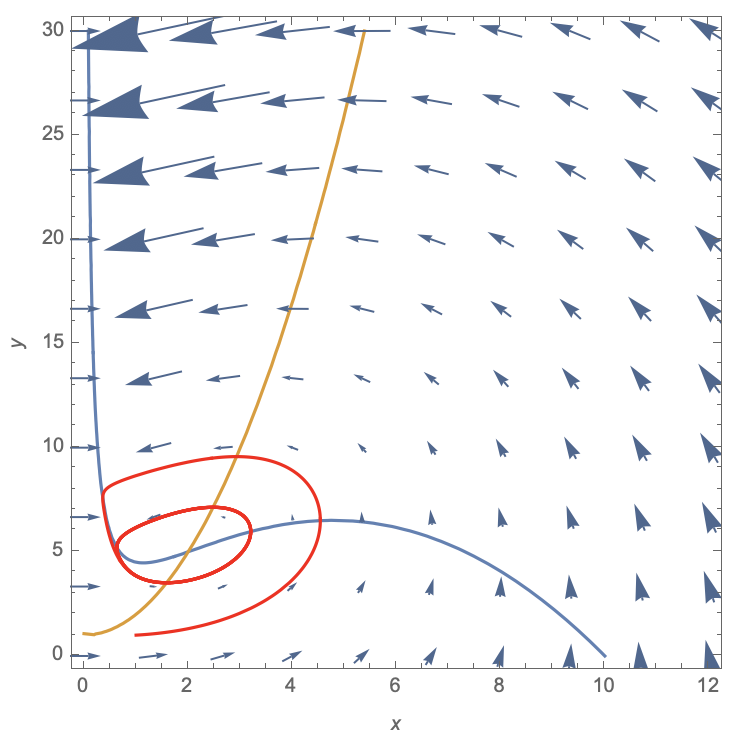
\includegraphics[scale=0.7]{img/C14trappingp1.png}

Consider the system 
\begin{align*}
\dot{r} = &\  r(2-\sin\theta -r) \\
\dot{\theta} = &\ 1.
\end{align*}

Show that the curve $r = 2-\sin\theta$ does not correspond to a trajectory of the system.

\vspace{0.2cm}
\hrule
\vspace{0.2cm}


\noindent \textbf{Extra vocabulary / extra facts:}
\begin{tcolorbox}
A \textbf{gradient system} is a dynamical system of the form $\dot{\underline{x}} = -\nabla V$ for a function $V(\underline{x})$.  In 2d, we have $\dot x = -V_x, \dot y = -V_y$.

For a gradient system, we call $V$ a \textbf{potential function}.

In a gradient system, trajectories flow perpendicular to the contours of $V$, and $V$ is \textbf{decreasing} along trajectories.  $\dot V = V_x \dot x + V_y \dot y = -V_x^2-V_y^2 \leq 0$ for all $(x,y)$ and $=0$ only when $V_x = V_y = 0$ (a fixed point).

When there exists a function $V$ that is decreasing along all trajectories that are not fixed points, there cannot be a closed orbit in the system.

It is sometimes possible to construct a function $V(x,y)$ such that $V(x,y)>0$ away from fixed points, $V(x,y) = 0$ at fixed points, and $V(x,y)$ is decreasing along non-fixed point trajectories.  Such a function is called a \textbf{Liapunov function}.
\end{tcolorbox}

\noindent\textbf{Examples}

Let $V = 2x^2 + y^2$.  

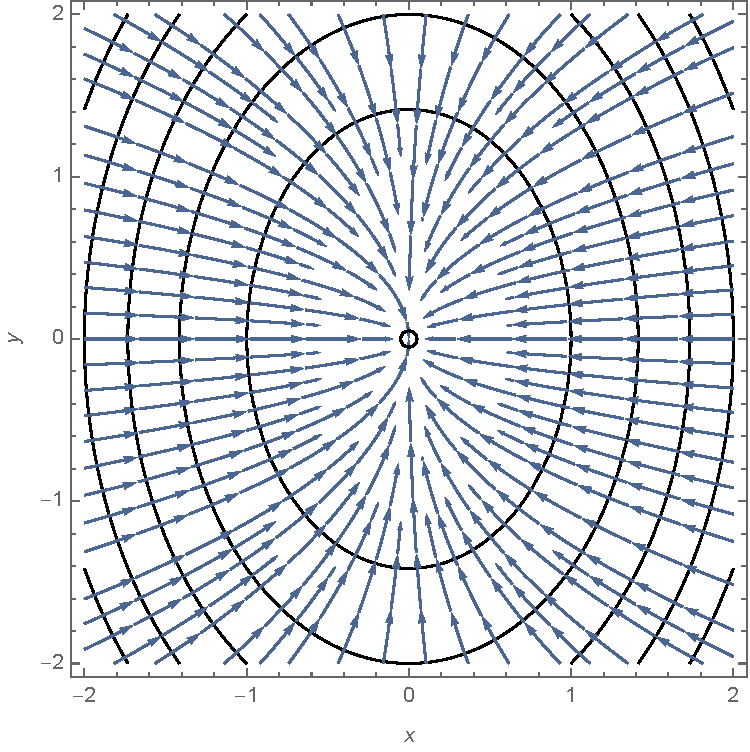
\includegraphics[width=3in]{img/C15gradient.pdf}

Let $\dot x = -x + 4y$, $\dot y = -x-y^3$.  This is not a gradient system.  Consider $V = x^2 + 4y^2$.  Show that this is a Liapunov function for this system.

\begin{itemize}
    \item $V(x,y)>0$ except at $(0,0)$.  $V(0,0) = 0$ and $(0,0)$ is the only fixed point.
    \item $\dot V = V_x \dot x + V_y\dot y = 2x(-x+4y) + 8y(-x-y^3) = -2x^2 -8y^4$
\end{itemize}


\begin{tcolorbox}
A \textbf{cylindrical phase space} arises when one coordinate can take on any value in $\mathbb{R}$ (the real numbers) while the other coordinate is an angle.

A \textbf{toroidal phase space} arises when two coordinates are angles.
\end{tcolorbox}

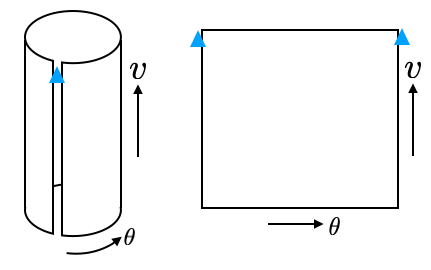
\includegraphics[width=0.5\textwidth]{img/191004p1.png}
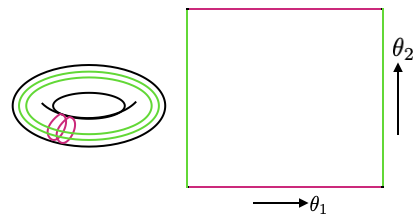
\includegraphics[width=0.5\textwidth]{img/191004p2.png}

\vspace{0.2cm}
\hrule
\vspace{0.2cm}


\noindent\textbf{Skill Check C16 practice}
\begin{questions}
\item All students who completed it satisfied Skill Check C13.  Optional retake of Skill Check C10 instead: classifying fixed points of linear systems based on $\tau$ and $\Delta$.

\item Consider the system $\dot r = r(1-r^2)+\mu r\cos\theta, \dot\theta = 1$.  Determine whether $r = 1$ is a phase curve of the system.

\vspace{0.2cm}

\hrule
\vspace{0.2cm}
\end{questions}



\noindent\textbf{Skill check C16 practice solution}

If $r-1 = 0$ is a phase curve then $\frac{d}{dt}(r-1) = 0$ when $r-1 = 0$.  We have $\frac{d}{dt}(r-1) = \dot r = r(1-r^2)+\mu r\cos\theta$.  On $r = 1$, this reduces to $\dot r = \mu\cos\theta$, which is only zero when $\mu = 0$, so $r=1$ is not a phase curve for $\mu\neq 0$.


\vspace{0.2cm}
\hrule
\vspace{0.2cm}





\eject



\vspace{0.2cm}

\hrule
\vspace{0.2cm}

\begin{questions}
\item The basic form of a differential equation describing the motion of a pendulum (with no damping) is $\displaystyle\ddot{\theta} = -A \sin \theta$.  For small $\theta$ this is often approximated as $\displaystyle\ddot{\theta} = -A\theta$.  This makes the system linear.  In this course, we're working with nonlinear systems, so we won't usually make that approximation.

\begin{parts}
\item For notational convenience, let $v = \dot{\theta}$ (the angular velocity).  Rewrite $\displaystyle\ddot{\theta} = - A \sin \theta$ as a system of two first order differential equations, $\dot{\theta} = ?, \dot{v} = ?$.
\item Consider the function $E(\theta,\dot{\theta}) = \frac{1}{2}(\dot{\theta})^2 - A \cos\theta$, or $E(\theta,v) = \frac{1}{2}v^2 - A \cos\theta$.  Show that $E(\theta,v)$ will be conserved on trajectories that satisfy $\displaystyle\ddot{\theta} = -A \sin \theta$.
% \item The function $E$ is called an \emph{energy function}.  The function $A\cos\theta$ is called the \emph{potential energy}.  Our text uses the notation $V(x)$ for the potential energy function (or $V(\theta)$ in this case).

% Show that $\displaystyle\ddot{\theta} = - A \sin \theta$ can be written as $\displaystyle\ddot{\theta} = - \frac{dV}{d\theta}$ for $V(\theta) = -A\cos\theta$.

% Notice that this notation is confusing: 
% \begin{itemize}
%     \item We used the notation $V(x)$ and the term \emph{potential function} for systems of the form $\dot{x} = -\frac{dV}{dx}$.
%     \item Now we're using the notation $V(x)$ and the term \emph{potential energy function} for systems of the form $\ddot{x} = -\frac{dV}{dx}$.
% \end{itemize}
% Sometimes a potential energy function may be referred to as a potential function, so it is important to figure out which kind of system is being referred to.

\item Our phase space is the angle-angular velocity space.  For our pendulum, this is the $\theta v$-space.  Use a rectangle to represent this phase space, but also draw the corresponding cylinder.

Think about how a pendulum moves.  Work to draw a trajectory in the phase space that corresponds to the motion of a pendulum without energy loss.  Draw it in each representation of your space.

\begin{itemize}
    \item There is a pendulum at the front of the room, but you can also use your (covered) marker as a pendulum.  
    \item Think of downwards as an angle of $0$.
    \item Let motion to the right have a positive angle and be the direction of positive velocity.
\end{itemize}

\item If the pendulum starts with a high enough positive velocity, it will swing all the way around.  Draw a trajectory that corresponds to this motion.

% \item How do you think the trajectory would look if the pendulum was losing energy, rather than energy being conserved?  Sketch a new trajectory for the pendulum with slow energy loss.

\end{parts}

\question To get used to a phase space that is a torus, think about two oscillators that are not interacting (like the hour hand and the minute hand on a clock: they each go at their own pace and that pace doesn't change).
\begin{parts}
\part Let $\dot\theta_1 = 1$ and $\dot\theta_2 = 2$.  If the oscillators each start at a phase angle of zero, so at the point $(0,0)$, draw their trajectory onto the phase space.  Use a square to represent the space.  Will the pair of oscillators pass through $(0,0)$ at some point?
\part Now let $\dot\theta_1 = \pi$ and $\dot\theta_2 = 2\pi$.  With an initial condition of $(0,0)$, draw their trajectory onto the phase space.  How is the trajectory different from the one in part a?
\part Let $\dot\theta_1 = \pi$ and $\dot\theta_2 = \sqrt{2}\pi$.  Assume the oscillator pair again starts at $(0,0)$.  The first oscillator will return to a phase of zero at time $2$, time $4$, etc.  When does the second oscillator return to a phase of zero?  Will the pair pass through $(0,0)$ at some point?
\end{parts}



% \begin{parts}
% \item Like last time, sketch a phase portrait for a system with a saddle point at the origin.
% \item Now add a stable spiral at $(1,0)$.  Connect the two local pictures up by having an (appropriate) unstable manifold of your saddle point spiral into the stable spiral.
% \item Could a closed trajectory exist in this system?  If so, where? 
% \end{parts}

% \textbf{Answer}:

% 1a: sketch of a saddle: two unstable directions, two stable ones, and those curvy trajectories.

% 1b: \includegraphics[width=4in]{img/S19C13p1.png}  Other configurations of the saddle point are possible, as is another orientation to the spin of the spiral.

% 1c: saddle point: index $-1$.  spiral: index $+1$.  both: index $0$.  So a closed trajectory would have to enclose just the spiral for the index to work out.  That isn't possible, because it would have to cross the unstable manifold of the saddle to do that.  No closed trajectories in this system!


\end{questions}

\textbf{Answers:} 
1a: $\dot{\theta} = v, \dot{v} = \ddot{\theta} = -A\sin\theta$. 

1b: $\frac{d}{dt}E = v \dot{v} -A(-\sin\theta)\dot{\theta} = v\dot{v} + vA\sin\theta = v(\dot{v} + A\sin\theta) = 0.$

1c: the trajectory should be an ellipse.  When $v>0$ we'll have $\theta$ increasing, so the arrow points clockwise.  Plots are on the back.

1d: This trajectory will have $v$ with the same sign at all times and will go all the way from one side to the other (one of the top two wavy trajectories on the plot on the left below).
\eject 

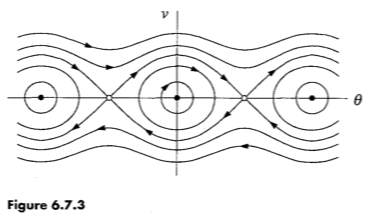
\includegraphics[width=4.5in]{img/191004p3.png}
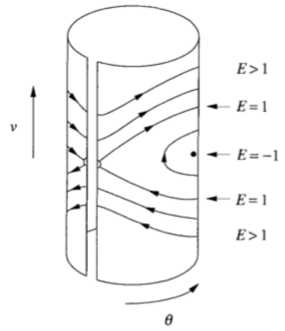
\includegraphics[width=2.5in]{img/191004p4.png}

%spiraling into the center (slowly)

2a: $\theta_1$ moves 1 unit in the time $\theta_2$ moves two units, so the trajectory is a line with slope $2$ through $(0,0)$.  It will leave at the top (at $(\pi,2\pi)$) and come back in at the bottom (at $(\pi,0)$). 

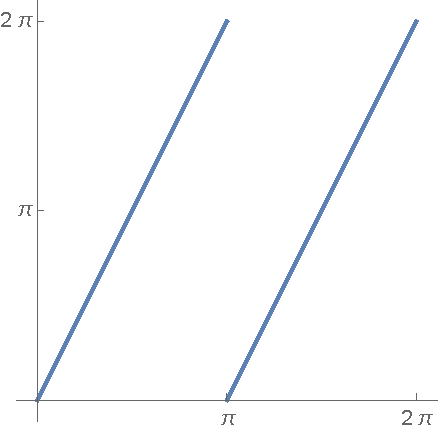
\includegraphics[width=2in]{img/191004p6.pdf}

2b: This trajectory will look the same as above.  We're just moving faster along the same path.

2c: The first oscillator returns at time $2$, time $4$, etc, so even positive integers.  The second oscillator returns to a phase of $0$ when the $\sqrt{2}\pi t = 2n\pi$ for $n$ an integer.  So when $\sqrt{2}t = 2n$ or when $t = \sqrt{2}n$.  These times are not integers.  The pair of oscillators will not pass through $(0,0)$ again!

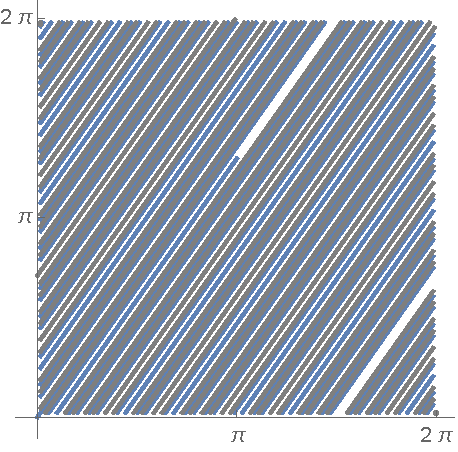
\includegraphics[width=2in]{img/191004p5.pdf}

\end{document}